
\documentclass[12pt]{article}
%%%\documentclass[12pt,a4paper]{scrartcl}
\usepackage[left=3cm,right=3cm,top=2cm,bottom=2cm]{geometry} % page settings
\usepackage{lingmacros}
\usepackage{tree-dvips}
\usepackage[polish]{babel}
%%% fix for \lll
\let\babellll\lll
\let\lll\relax 
\usepackage[T1]{fontenc}


\usepackage{amssymb}
\usepackage{verbatim}
\usepackage{listings}
\usepackage{amsmath}
\usepackage{amsthm}
\usepackage[boxed]{algorithm2e}
\usepackage{float}
\usepackage{graphicx}
\usepackage{csvsimple}
\usepackage{pgfplotstable}

\renewcommand{\algorithmcfname}{Algorytm}
\SetKwInput{KwData}{\textbf{Dane}}
\SetKwInput{KwResult}{\textbf{Wynik}}
\renewcommand{\qedsymbol}{$\blacksquare$}

\title{Zadanie 4}
\author{Marko Golovko}
\date{\today}

\begin{document}
\maketitle

\section*{Przygotowanie danych}
Ze strony www.populationpyramid.net, pobrałem dane dla 20 krajów (dane z dnia 14.05.2020). Program, który zawiera się w csv$\_$convert.py tworzy tabelę z 10-letnimi przedziałami czasowymi dla ludności ogółem.\\
\\
Dla przykładu część tabeli. Wierszy odpowiadają za przedziały czasowe od 0-9 do 100+. Cała tablica znajduje się w pliku CountriesPopulation.csv.
\\
\\
\pgfplotstabletypeset[col sep=comma,
     columns={RUS, ESP, UK, ITA, GER, TUR, FRA, BEL},
    ]{CountriesPopulation.csv}
\\
\\
W pliku dane0512.ods znajduję się łączna liczba zachorowań w tych krajach oraz liczba zgonów.

\section*{Teoria}

\subsection*{Regresja (względem) wielu zmiennych.}
Dane są niezależne obserwacje $(x_{i1},x_{i2},\ldots,x_{ik},y_{i})$, dla $i = 1,\ldots,n$.
Szukamy wektor $\beta=[\beta_{0},\beta_{1},\ldots,\beta_{k}]$ minimalizujący wartość funkcji
$$ f(\beta)=\sum_{i=1}^{n}
(\beta_{0}+\beta_{1}x_1+\ldots+\beta_{k}x_k-y_i)^2.$$
Gdzie $n$ to ilość krajów. $y_i$ łączna liczba zachorowań w i-tym kraju lub łączna liczba zgonów w zależności od przypadku. $x_{ik}$ liczba ludzi w i-tym kraju i k-tym przedziale ($x_1$ to $0-9,\ldots, x_{10}$ to $100+$).\\
Przechodząc do wersji macierzowej.
$$
\left[ \begin{array}{ccccc}
1 & x_{11} & x_{12} & \ldots & x_{1k}\\
1 & x_{21} & x_{22} & \ldots & x_{2k}\\
\vdots & \vdots & \vdots & \ddots & \vdots \\
1 & x_{n1} & x_{n2} & \ldots & x_{nk}
\end{array} \right]
\quad
\left[ \begin{array}{c}
\beta_0\\
\vdots \\
\beta_k
\end{array} \right]
\approx
\left[ \begin{array}{c}
y_1\\
y_2\\
\vdots \\
y_n\\
\end{array} \right]
$$
Mnożąć powyższą równość lewostronnie, przez $X^T$ otrzymujemy
$$ X^TX\beta=X^TY$$
I obliczamy wektor
$$ \beta=( X^TX)^{-1}X^TY $$

\section*{Obliczenia i wnioski}
\subsection*{Wyniki obliczeń}
Obliczenia są zapisane w pliku dz4.py. Pokazuję tylko końcowy wynik ze względu na rozmiar macierzy otrzymanych w pośrednich obliczeniach. \\
Dla równania regresji zachorowań 
$$ \beta_c^T = [-4835\quad 0.1084 \quad  -0.1332\quad 0.0378\quad  -0.0839\quad 0.0679\quad 0.0637\quad -0.029\quad 0.0182\quad $$ 
$$-0.1395\quad 0.2332 \quad 0.7787 ] $$
\\
Dla równania regresji zgonów 
$$ \beta_d^T = [-2493\quad 0.0102\quad -0.0093 \quad -0.0026 \quad  -0.0048 \quad 0.0057 \quad  0.0048 \quad  -0.0102 \quad  0.0243 $$
$$\quad -0.0345 \quad 0.1064 \quad -2.5124 ] $$
\cleardoublepage

\begin{figure}[hbt!]
\subsection*{Wnoiski}
Wizualizując obliczenia, otrzymałem takie dwa wykresy.
\centering zachorowania i zgony
 \centering
 \caption{Zachorowania}
 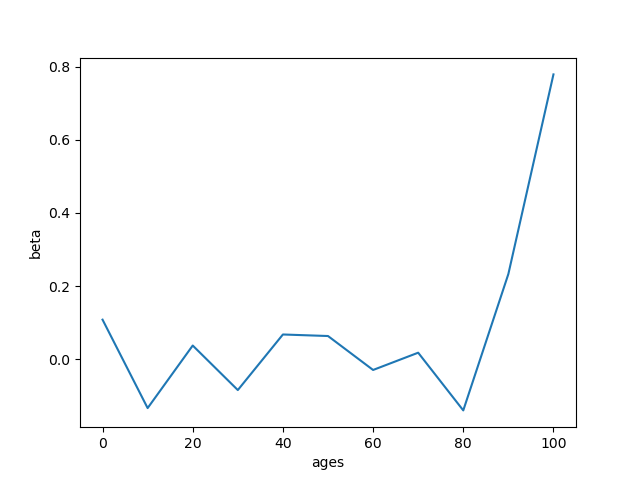
\includegraphics[width=0.8\textwidth]{cases}
 \caption{Zgony} 
 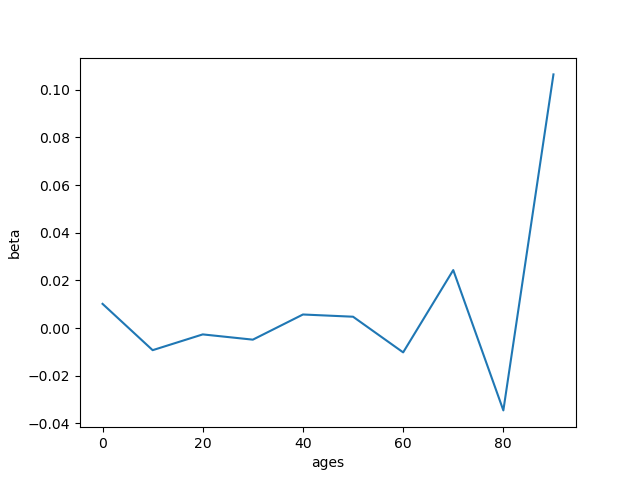
\includegraphics[width=0.8\textwidth]{deaths}
 \begin{flushleft}
 Z wykresów wynika przypuszczenie, że dla osób w wieku więcej od 60, zwiększa się ryzyko.
 \end{flushleft} 
\end{figure}

\end{document}